\chapter{Background and/or status of the matter}

Nowadays, there are many solutions that can fit to solve our problem. Some are very expensive, and others have shortcomings. In this chapter, we will have a look at some of the most popular solutions.

\section{Smaart}

\textbf{Smaart}, an acronym for \textit{System Measurement Acoustic Analysis Real-time Tool} \cite{SMAART}, is a software-based solution commercialized by Rational Acoustics. It is probably the most used and well-known solution for professional acoustic analysis, used in big venues, concert halls, stadiums, touring productions, as well as in professional audio studios and speaker development laboratories.  Common uses are:

\begin{itemize}
	\item \textbf{Speaker Alignment:} When we have multiple sound sources, this software helps us find the phase and delay between them. For example, it can be used to find the time and phase alignment between a subwoofer and a full-range speaker.
	
	\item \textbf{RTA, Frequency and Phase Response} used to view live spectrograms, phase deviation, or energy in frequency bands. One example of use is identifying resonances at specific frequencies.

	\item \textbf{Coherence Analysis} to evaluate the quality of the measured data. A common use is to detect reflections and background noise.
	
	\item \textbf{Delay Time} between different sources or signals. Widely used to synchronize different elements of the system.
	
	\item \textbf{Room and architectural acoustics} to identify the frequency and phase response of a room, as well as reverberation and echoes.
\end{itemize}
	
\begin{figure}[H]
	\centering
	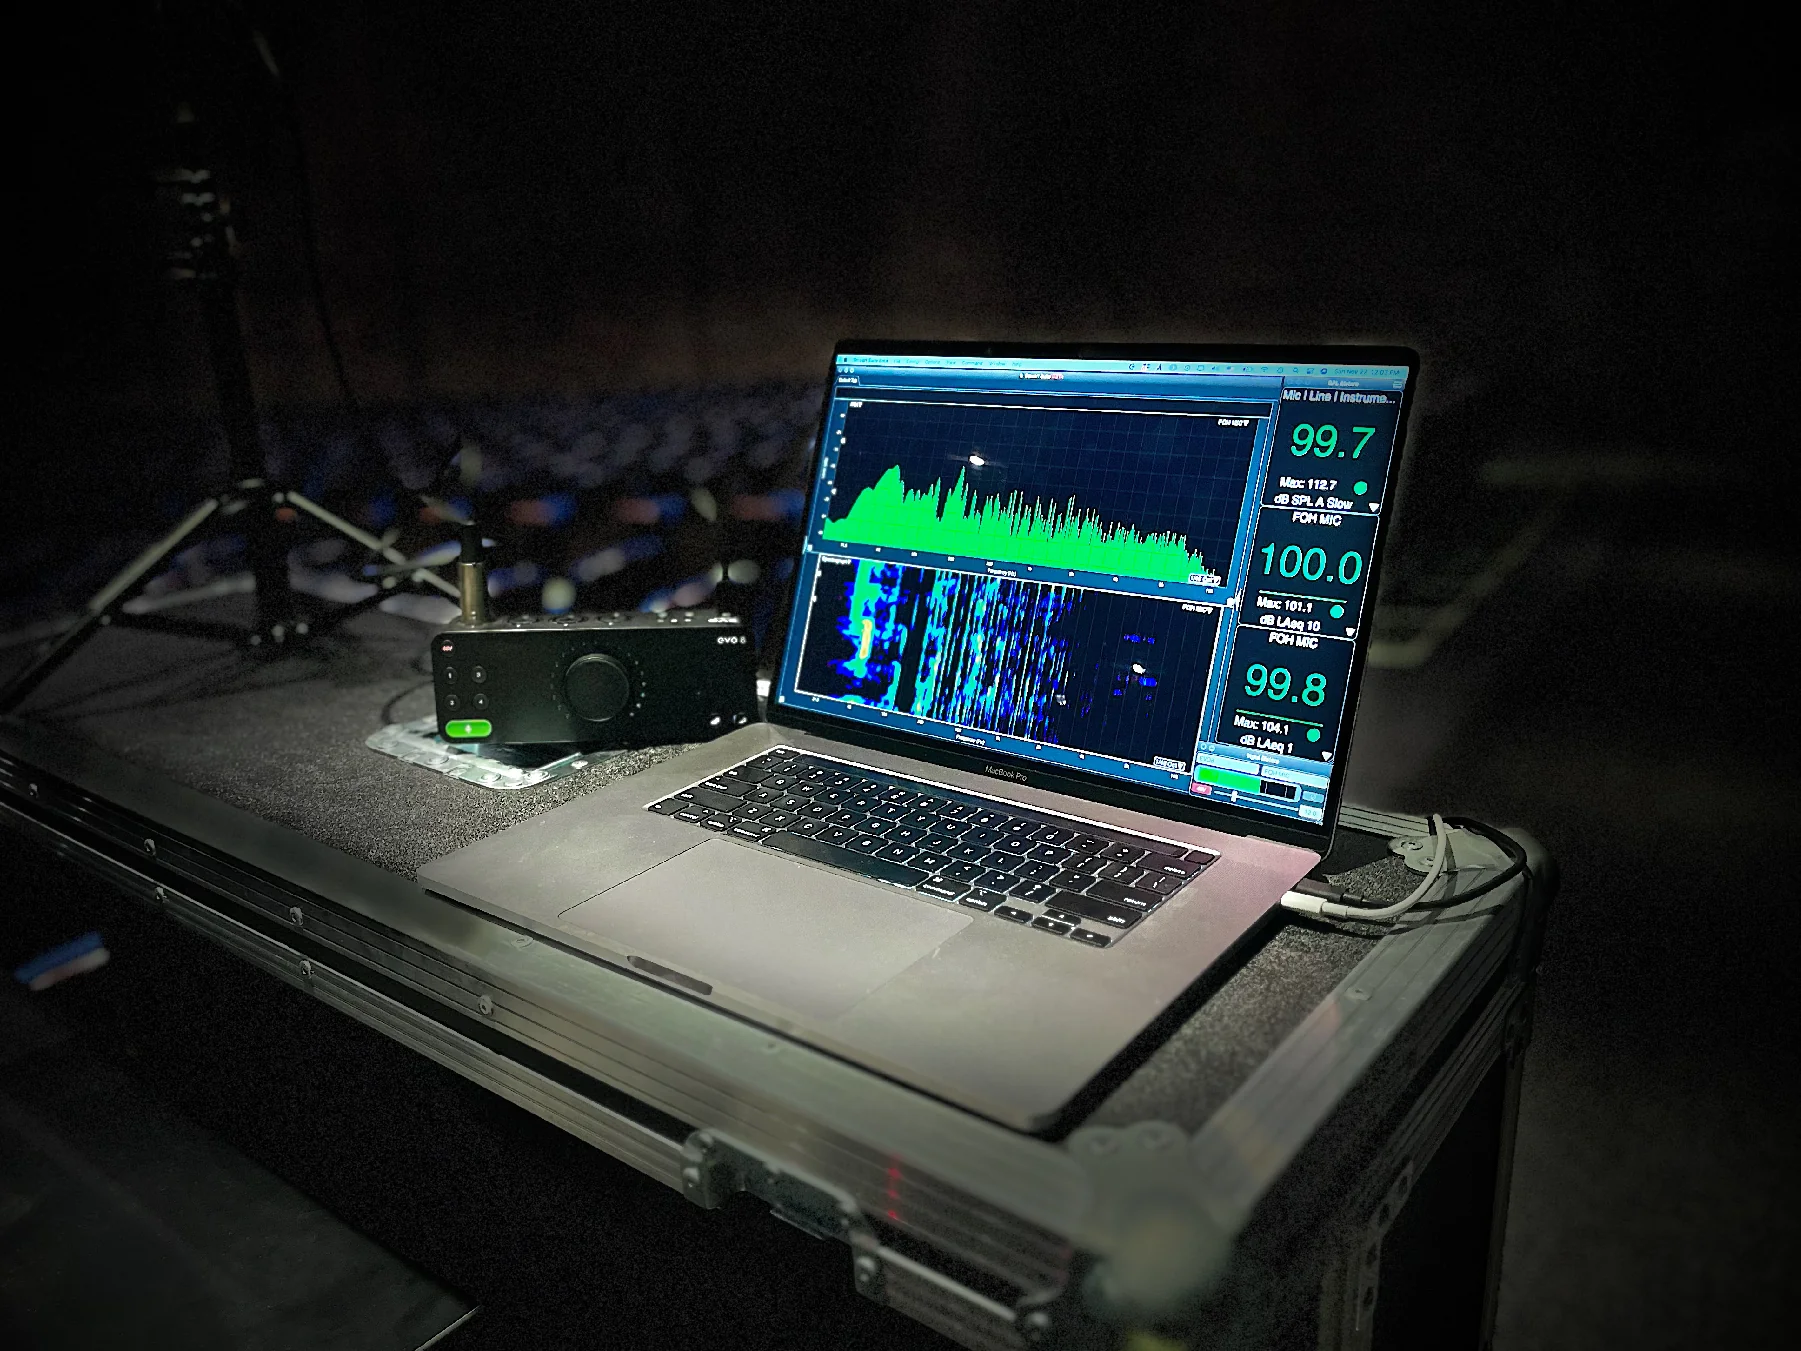
\includegraphics[width=0.9
	\linewidth]{Figures/smaart_01.png}
	\caption{Notebook using Smaart, where we can see some of the tools it includes. The notebook is connected to the EVO 8 (a USB interface that acts as an external sound card).}
	\label{fig:SMAART}
\end{figure}

	
The strongest points of this program are:

\begin{itemize}
	\item \textbf{Flexibility:} As a software-based solution, it can run on any Windows or Mac computer (meeting the minimum required specs}), and can be used with most external audio sound cards, allowing the connection of unlimited types of microphones or direct signals.
	
	\item \textbf{More than one channel:} This software can analyze and display information from more than one input channel at the same time, allowing comparisons between different channels. This is used to compare an original signal with the signal captured by a microphone inside a room with a sound system, helping to detect room acoustics or sound system issues. Another common use is to measure the sound in different places of the same room simultaneously.
	
	\item \textbf{Widely used:} It is very common to see professionals in the sector using this software, or at least being familiar with it. It has become a kind of standard, which leads other companies to ensure maximum compatibility with it. For example, Audix makes the Audix TM-1 Plus microphone \cite{AudixTM1}, which includes a file that can be imported into SMAART to apply microphone correction during analysis.
\end{itemize}

On the other hand, it requires a license, external hardware such as sound cards and microphones, and it does not have any correction capabilities—only analysis.


\section{Dirac} Home correction solution -----------------------------------------------------------------

\section{REW} Free software for room measurement ---------------------------------------------------------

\section{Trinnov} Hardware base solution with correction -------------------------------------------------








******************************** Exemple d'esquema *************************************

\begin{center}
\vspace{-2mm}
\tikzsetnextfilename{vad_fsa_basico}
\begin{tikzpicture}[node distance=30mm,on grid,auto, scale=1, bend angle=45]
	% \draw[help lines] (0,0) grid (3,2);
	every node/.style={font=\small};
	
	\node (q_init) {start};
	\node (null_init) [right=of q_init] {};
	\node[state, minimum size=15mm] (q_sil) [above right=of null_init] {silence};
	\node[state, minimum size=15mm] (q_voice) [below right=of null_init] {voice};
	\node (null_final) [above right=of q_voice] {};
	\node (q_final) [right=of null_final] {end};
	
	
	\draw[blue, dotted, very thick, ->] (q_init) edge node {} (q_sil);
	\draw[blue, dotted, very thick, ->] (q_init) edge node {} (q_voice);
	\draw[blue, dotted, very thick, ->] (q_sil) edge node {} (q_final);
	\draw[blue, dotted, very thick, ->] (q_voice) edge node {} (q_final);
	
	\path[->,every node/.style={font=\footnotesize}]
	(q_sil) edge [bend left, thick] node {$C_{S,V}$} (q_voice)
	edge [loop above, thick] node {$C_{S}$} ()
	(q_voice) edge [bend left, thick] node  {$C_{V,S}$} (q_sil)
	edge [loop above, thick] node {$C_{V}$} ()
	;
\end{tikzpicture}
\vspace{-2mm}
\end{center}